% ------------------------------------------------------------------------------
% ANEXO
% Existe adicionalmente el entorno \begin{appendixd} que permite insertar
% \chapter y el entorno \begin{appendixdtitle}[style1] (4 estilos diferentes),
% el cual acepta \chapter y escribe el título de anexos encima
% ------------------------------------------------------------------------------
\begin{appendixs}
	
	\section{Additional DDPO samples}\label{appendix:additional-samples}

    % \textbf{Additional samples.} A hundred additional comparable samples from the pretrained and DDPO finetuned models are provided.

        % 100 samples from the pretrained model
        \begin{figure}[ht]
            \centering
            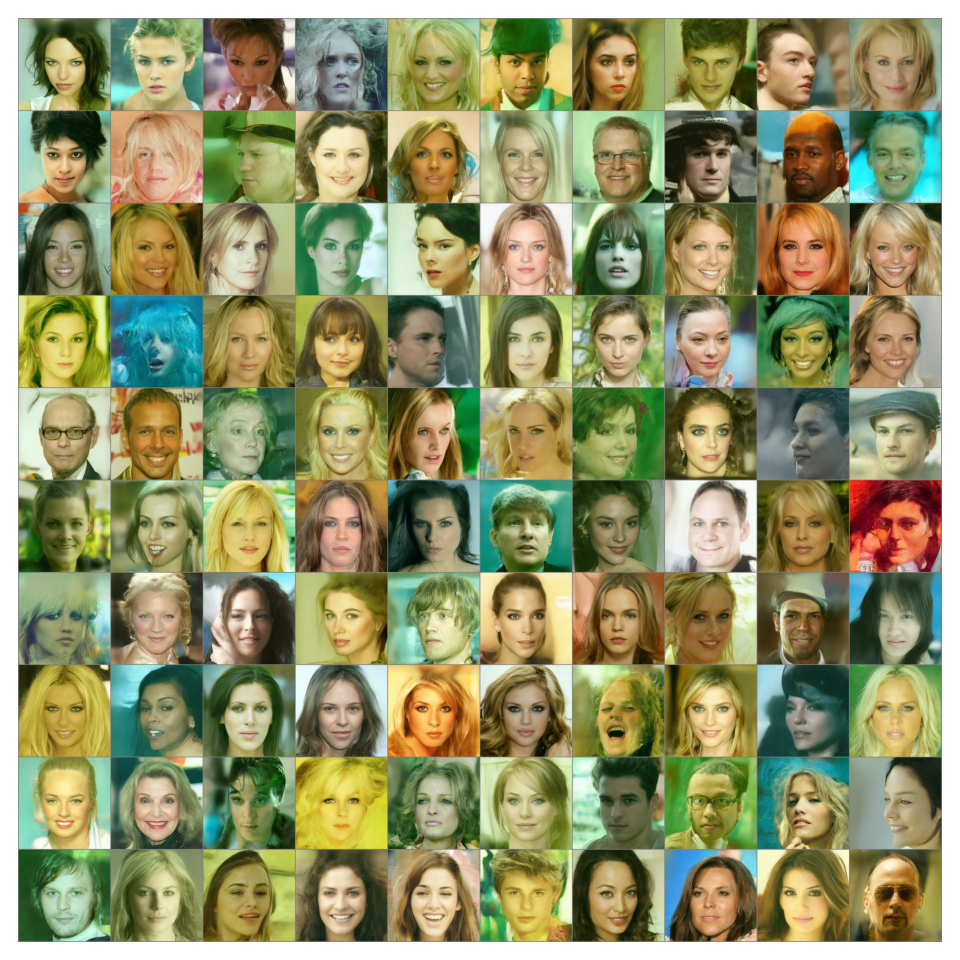
\includegraphics[scale=0.8]{img/results/ddpm-samples.png}
            \vspace{-4pt}  % reduce space between caption and figure
            \captionsetup{width=\textwidth} % set the width of the caption
            \caption{Celeba-HQ 256x256 generated samples from the pretrained model google/ddpm-celebahq-256.}
            \label{fig:ddpm-samples}
        \end{figure}

        % 100 samples from the finetuned model with ddpo and compressibility
        \begin{figure}
            \centering
            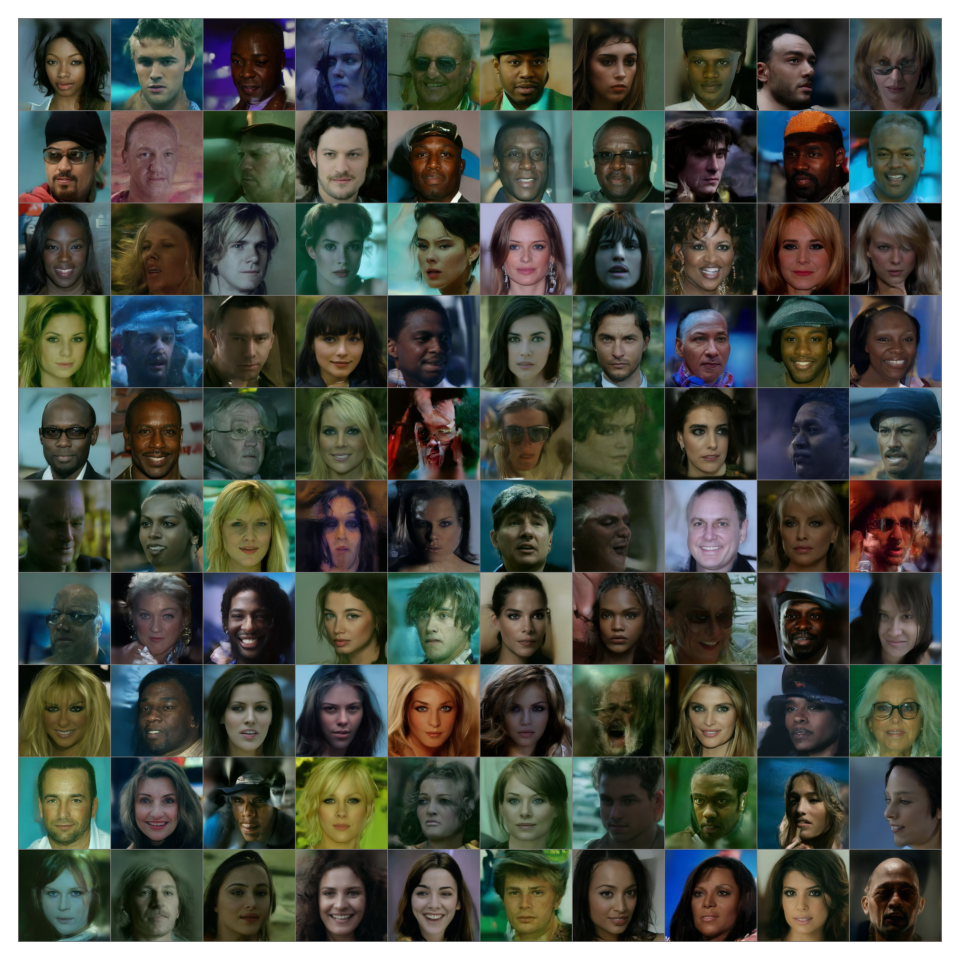
\includegraphics[scale=0.8]{img/results/ddpo-compressibility-samples.png}
            \vspace{-4pt}  % reduce space between caption and figure
            \captionsetup{width=\textwidth} % set the width of the caption
            \caption{Celeba-HQ 256x256 generated samples from the DDPO finetuned model optimized by JPEG compressibility.}
            \label{fig:ddpo-compressibility-samples}
        \end{figure}

        % 100 samples from the finetuned model with ddpo and incompressibility
        \begin{figure}
            \centering
            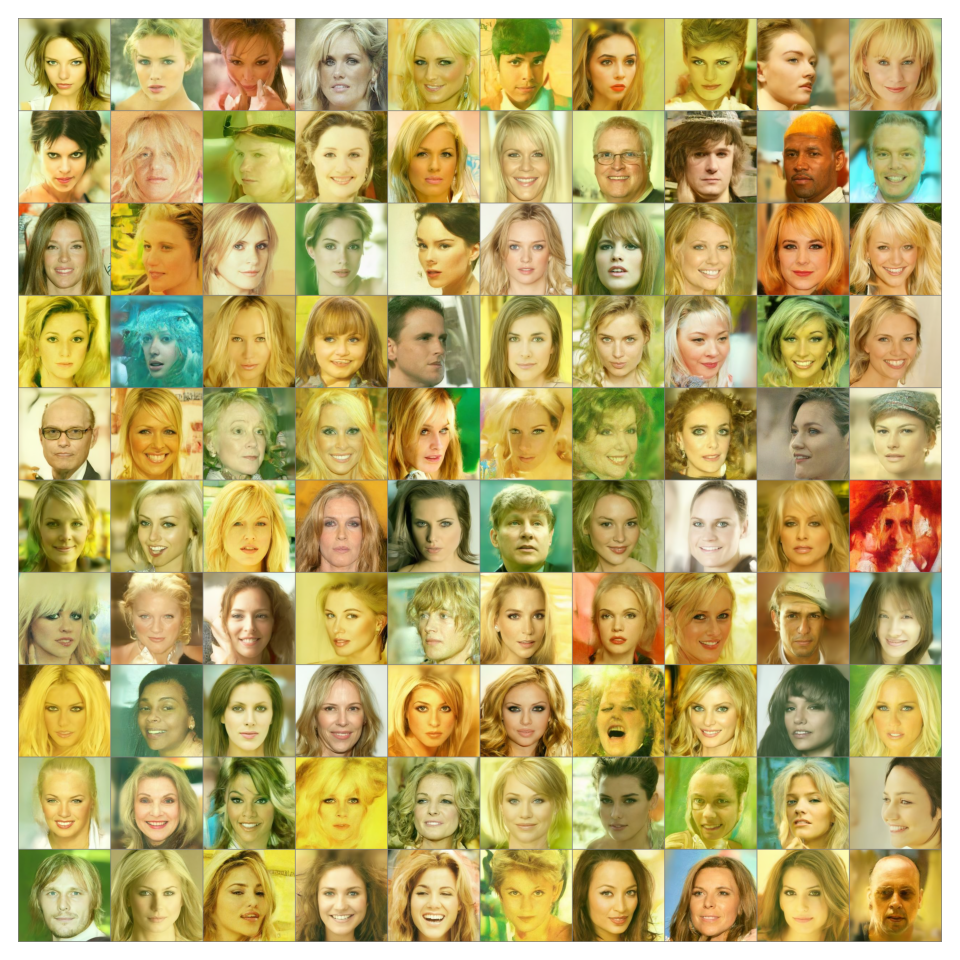
\includegraphics[scale=0.8]{img/results/ddpo-incompressibility-samples.png}
            \vspace{-4pt}  % reduce space between caption and figure
            \captionsetup{width=\textwidth} % set the width of the caption
            \caption{Celeba-HQ 256x256 generated samples from the DDPO finetuned model optimized by JPEG incompressibility.}
            \label{fig:ddpo-incompressibility-samples}
        \end{figure}

        % 100 samples from the finetuned model with ddpo and aesthetic quality
        \begin{figure}
            \centering
            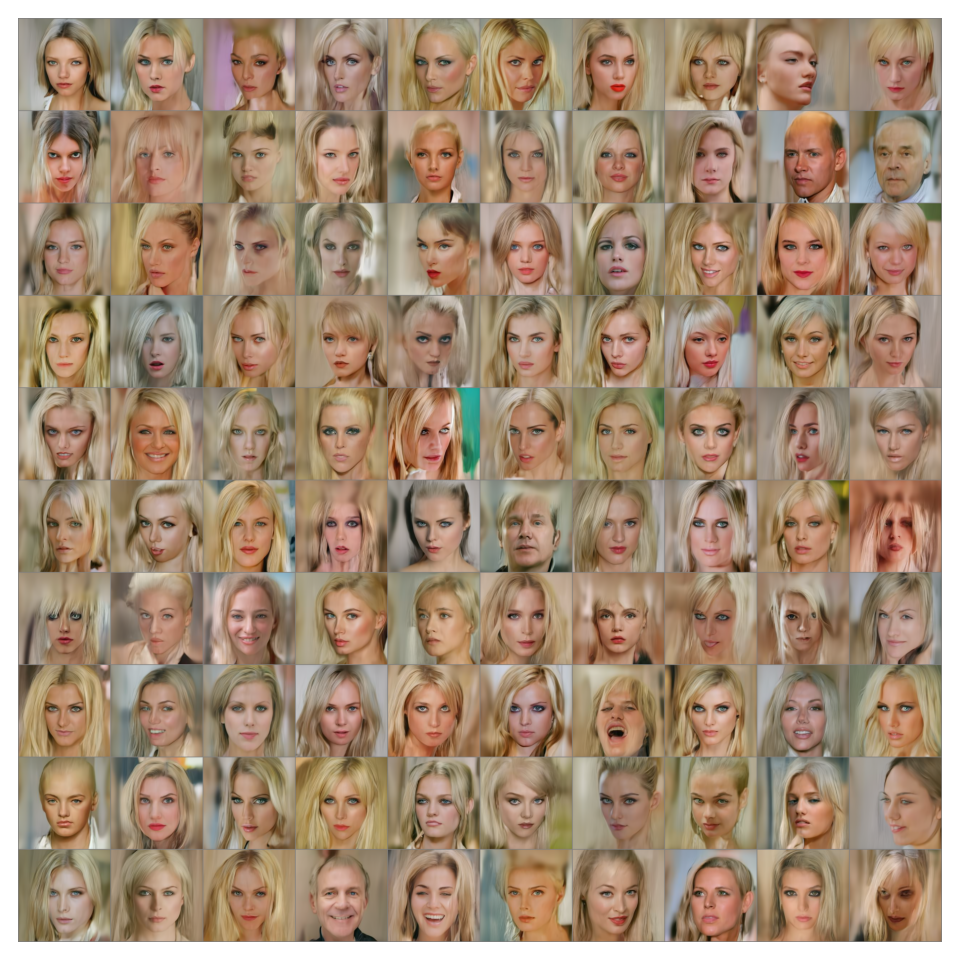
\includegraphics[scale=0.8]{img/results/ddpo-aesthetic-samples.png}
            \vspace{-4pt}  % reduce space between caption and figure
            \captionsetup{width=\textwidth} % set the width of the caption
            \caption{Celeba-HQ 256x256 generated samples from the DDPO finetuned model optimized by aesthetic quality.}
            \label{fig:ddpo-aesthetic-samples}
        \end{figure}

    \newpage

    \section{Additional transitions from DDPM to DDPO}

        % transition using jpeg compressibility extra sample 1
        \begin{figure}
            \centering
            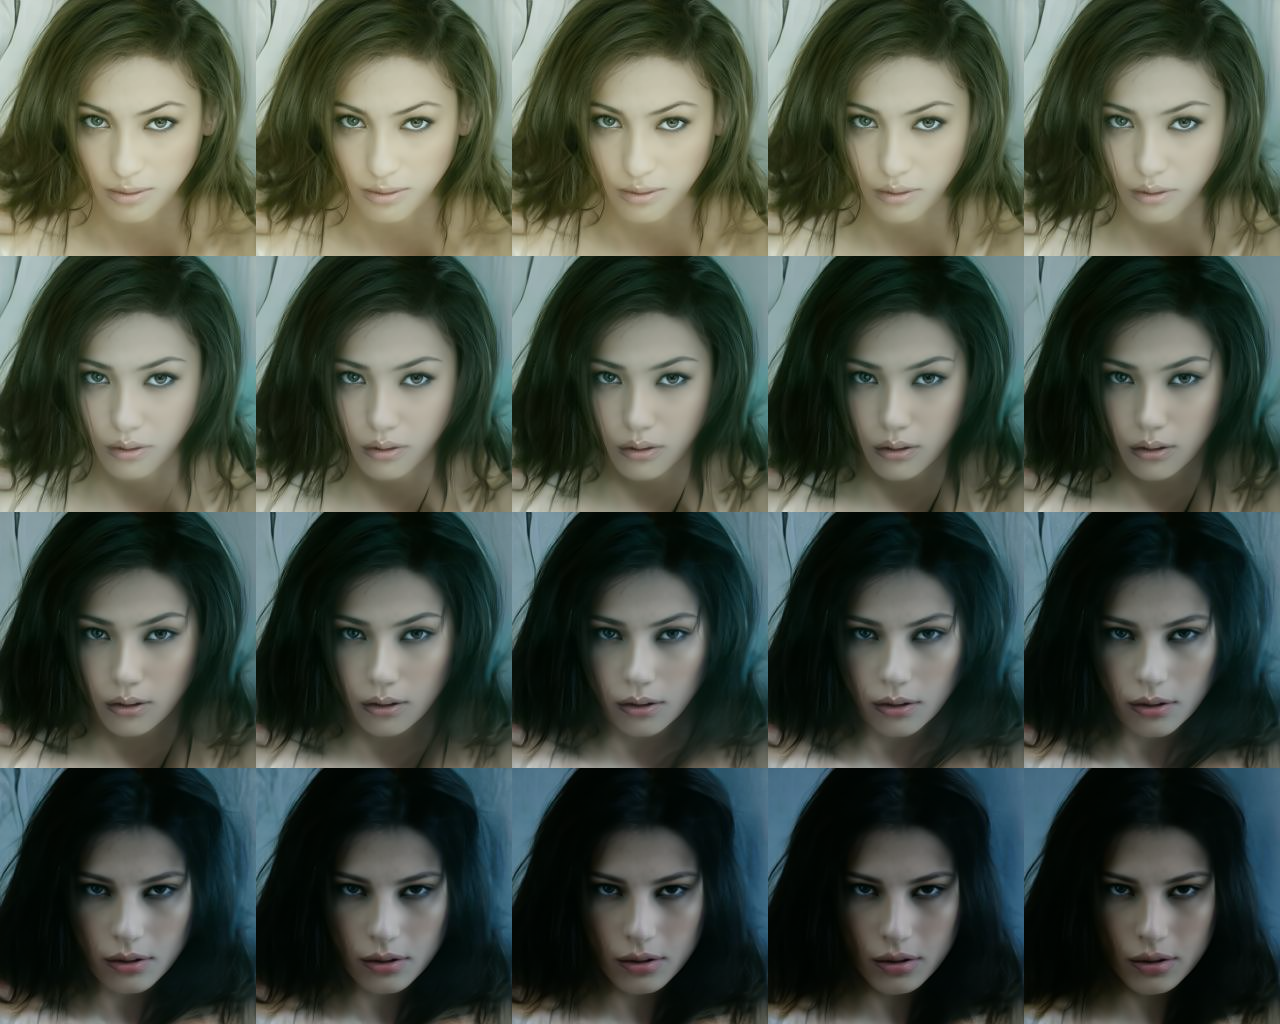
\includegraphics[scale=1.40]{img/results/compressibility_40.png}
            \vspace{-0pt}  % reduce space between caption and figure
            \captionsetup{width=\textwidth} % set the width of the caption
            \caption{\textbf{Additional example 1 of JPEG compressibility transformation during model updates}, starting from a pretrained DDPM model and optimized to maximize the reduction in image filesize after JPEG compression using DDPO.}
            \label{fig:ddpm-to-ddpo-compressibility-extra1}
        \end{figure}

        % transition using jpeg compressibility extra sample 2
        \begin{figure}
            \centering
            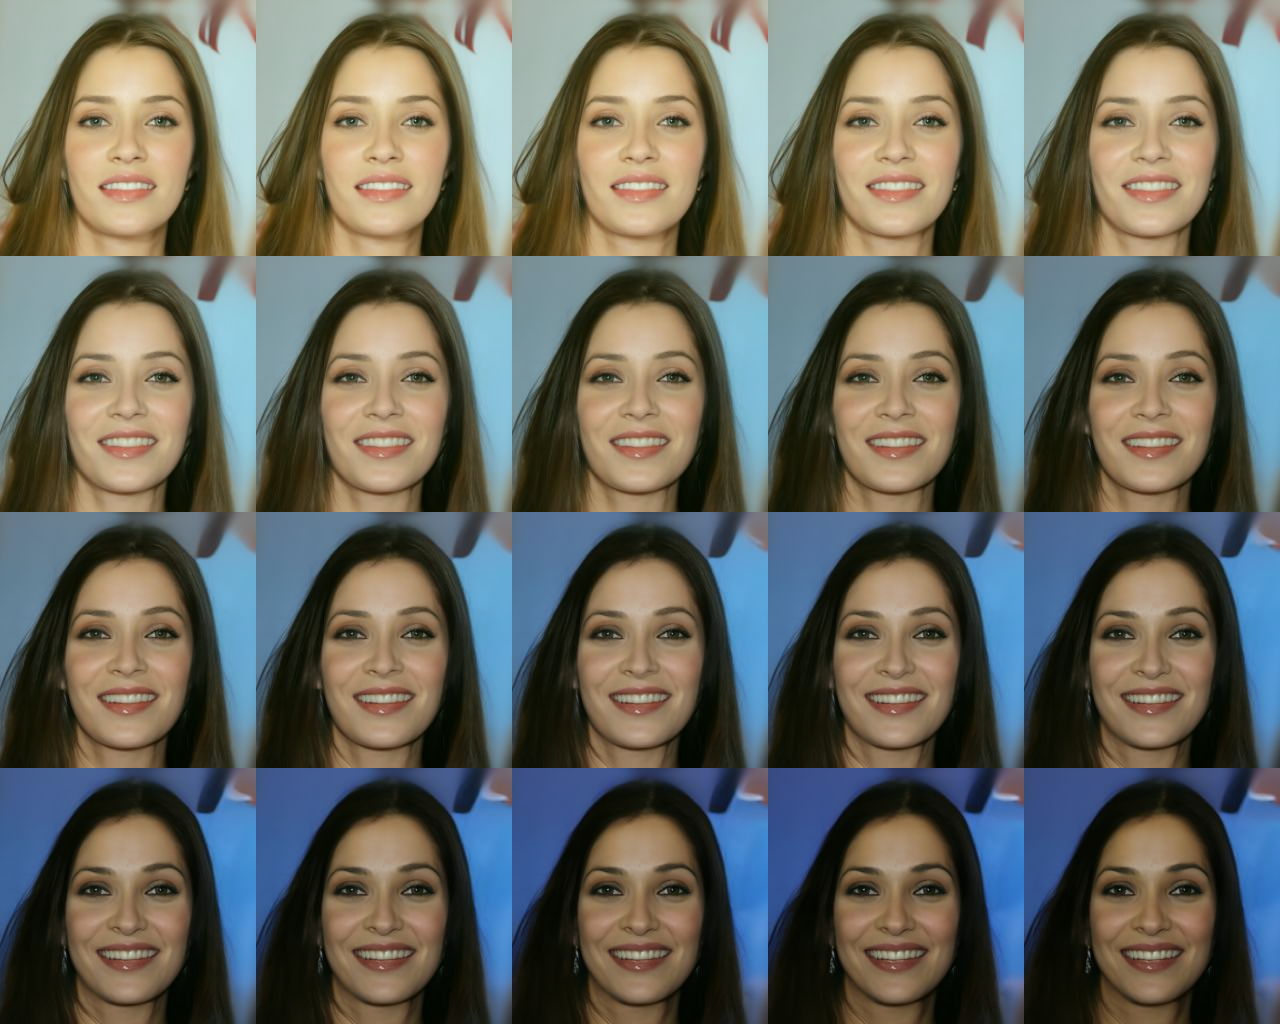
\includegraphics[scale=1.40]{img/results/compressibility_44.png}
            \vspace{-0pt}  % reduce space between caption and figure
            \captionsetup{width=\textwidth} % set the width of the caption
            \caption{\textbf{Additional example 2 of JPEG compressibility transformation during model updates}, starting from a pretrained DDPM model and optimized to maximize the reduction in image filesize after JPEG compression using DDPO.}
            \label{fig:ddpm-to-ddpo-compressibility-extra2}
        \end{figure}

        % transition using jpeg incompressibility extra sample 1
        \begin{figure}
            \centering
            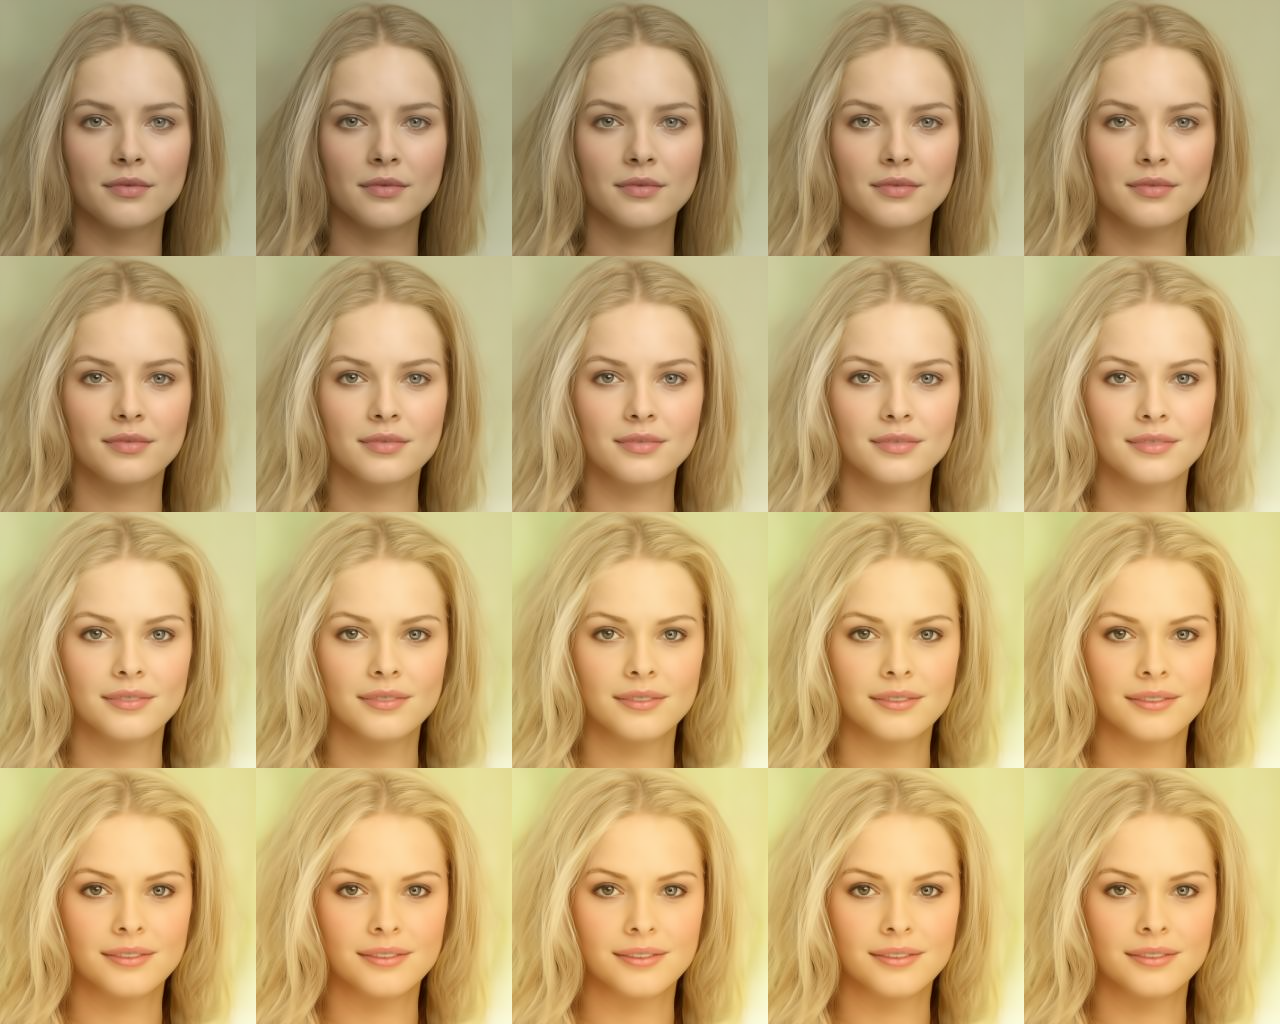
\includegraphics[scale=1.40]{img/results/incompressibility_8.png}
            \vspace{-0pt}  % reduce space between caption and figure
            \captionsetup{width=\textwidth} % set the width of the caption
            \caption{\textbf{Additional example 1 of JPEG incompressibility transformation during model updates}, starting from a pretrained DDPM model and optimized to increase the image filesize after JPEG compression using DDPO.}
            \label{fig:ddpm-to-ddpo-incompressibility-extra1}
        \end{figure}


        % transition using jpeg incompressibility extra sample 2
        \begin{figure}
            \centering
            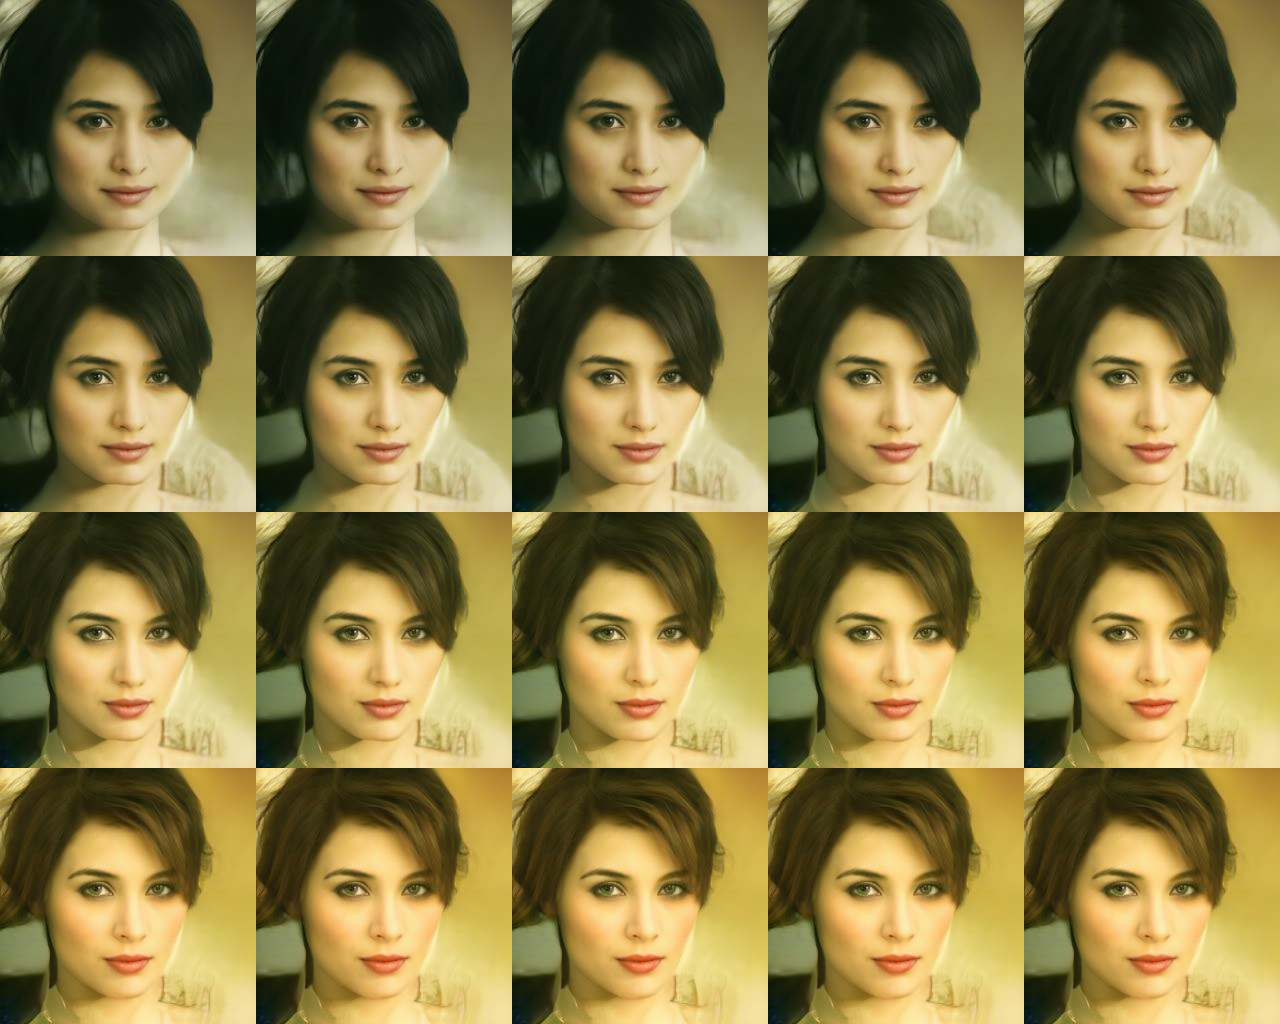
\includegraphics[scale=1.40]{img/results/incompressibility_28.png}
            \vspace{-0pt}  % reduce space between caption and figure
            \captionsetup{width=\textwidth} % set the width of the caption
            \caption{\textbf{Additional example 2 of JPEG incompressibility transformation during model updates}, starting from a pretrained DDPM model and optimized to increase the image filesize after JPEG compression using DDPO.}
            \label{fig:ddpm-to-ddpo-incompressibility-extra2}
        \end{figure}

        % transition using aesthetic quality extra sample 1
        \begin{figure}
            \centering
            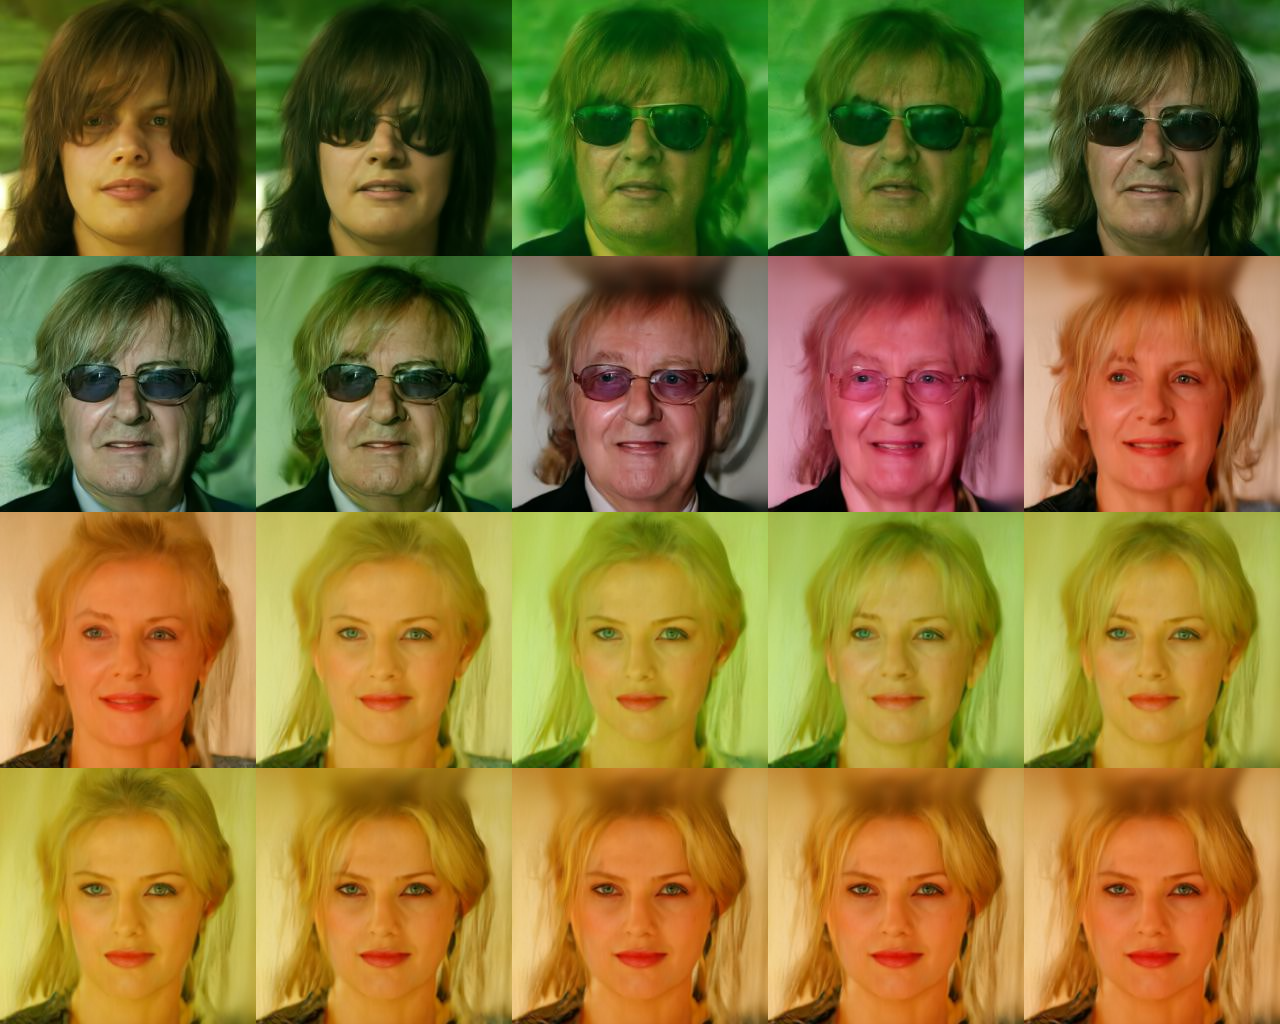
\includegraphics[scale=1.40]{img/results/laion_1.png}
            \vspace{-0pt}  % reduce space between caption and figure
            \captionsetup{width=\textwidth} % set the width of the caption
            \caption{\textbf{Additional example 1 of aesthetic quality transformation during model updates}, starting from a pretrained DDPM model and optimized to maximize the LAION aesthetic score using DDPO.}
            \label{fig:ddpm-to-ddpo-aesthetic-extra1}
        \end{figure}


        % transition using aesthetic quality extra sample 2
        \begin{figure}
            \centering
            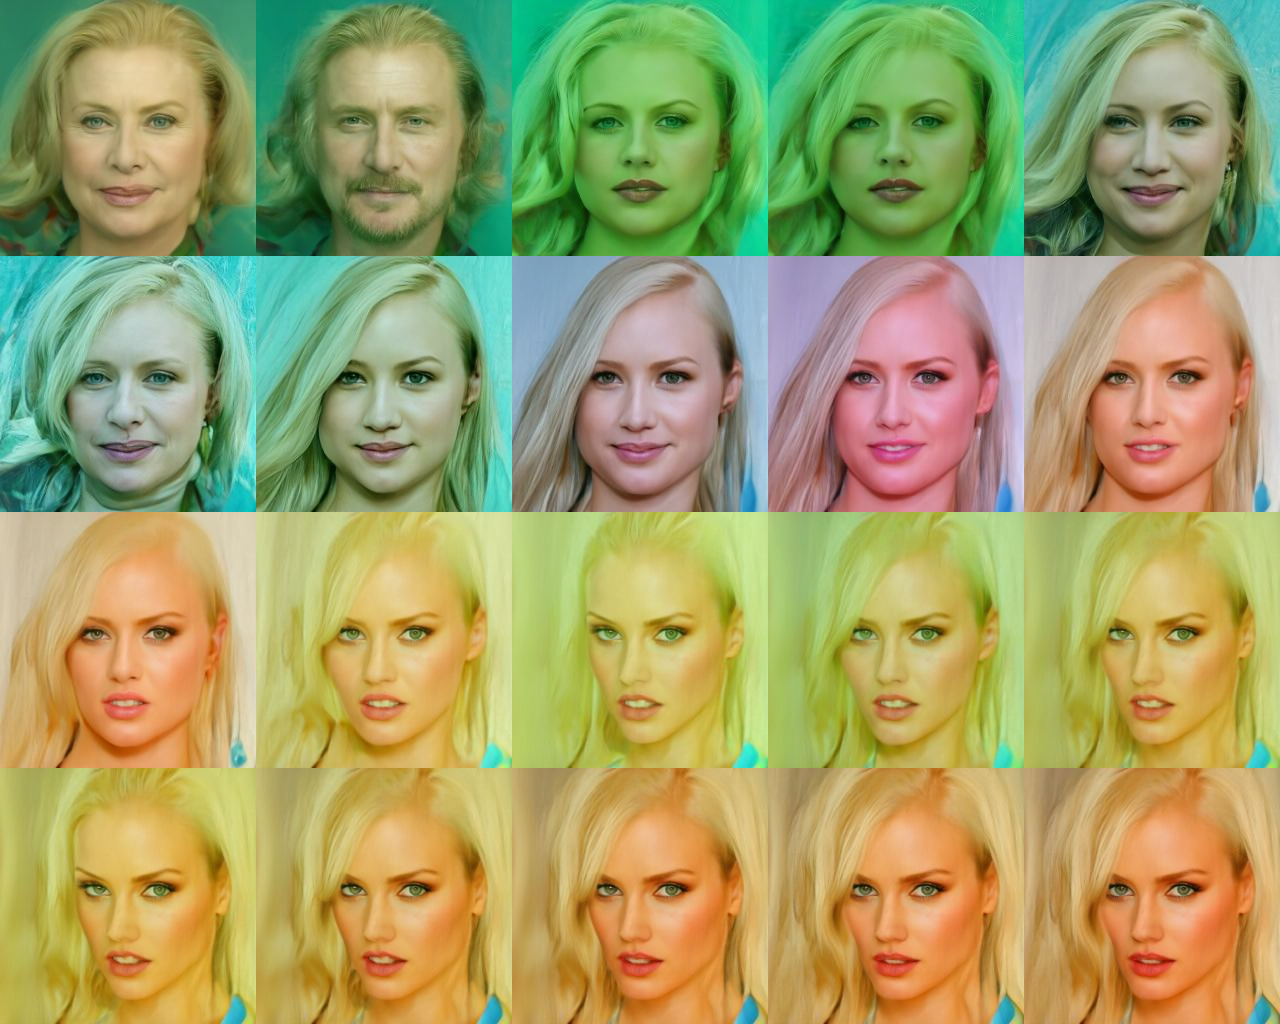
\includegraphics[scale=1.40]{img/results/laion_12.png}
            \vspace{-0pt}  % reduce space between caption and figure
            \captionsetup{width=\textwidth} % set the width of the caption
            \caption{\textbf{Additional example 2 of aesthetic quality transformation during model updates}, starting from a pretrained DDPM model and optimized to maximize the LAION aesthetic score using DDPO.}
            \label{fig:ddpm-to-ddpo-aesthetic-extra2}
        \end{figure}

        % transition from DDPM to DDPO samples optimized for Task.OVER50 (ViT age classifier) extra sample 1
        \begin{figure}
            \centering
            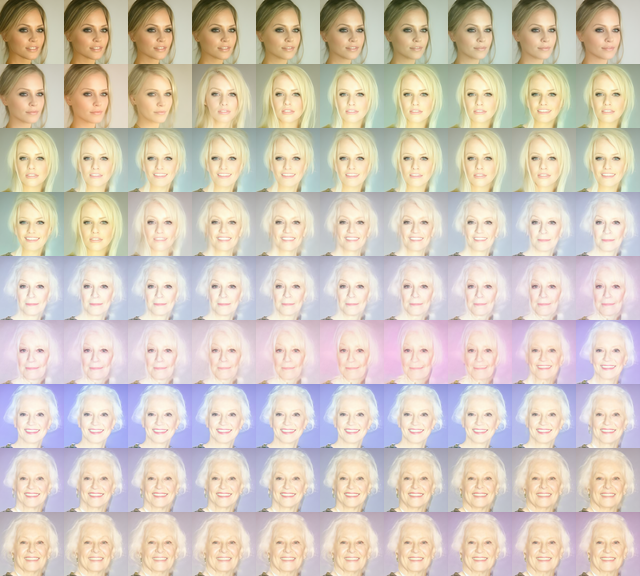
\includegraphics[scale=2.80]{img/results/over50_7.png}
            \vspace{-0pt}  % reduce space between caption and figure
            \captionsetup{width=\textwidth} % set the width of the caption
            \caption{\textbf{Additional example 1 of OVER50 transformation during model updates}, starting from a pretrained DDPM model and optimized to maximize the sum of logits for classes ≥ 50 years old of the ViT Age classifier using DDPO.}
            \label{fig:ddpm-to-ddpo-over50-extra1}
        \end{figure}

        % transition from DDPM to DDPO samples optimized for Task.OVER50 (ViT age classifier) extra sample 2
        \begin{figure}
            \centering
            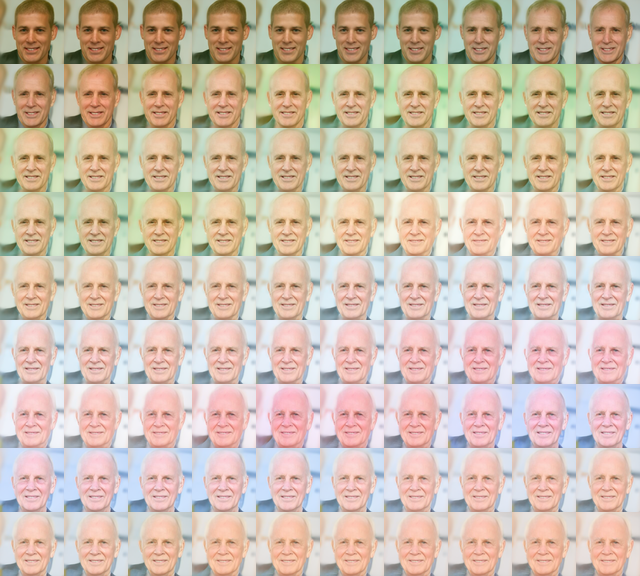
\includegraphics[scale=2.80]{img/results/over50_46.png}
            \vspace{-0pt}  % reduce space between caption and figure
            \captionsetup{width=\textwidth} % set the width of the caption
            \caption{\textbf{Additional example 2 of OVER50 transformation during model updates}, starting from a pretrained DDPM model and optimized to maximize the sum of logits for classes ≥ 50 years old of the ViT Age classifier using DDPO.}
            \label{fig:ddpm-to-ddpo-over50-extra2}
        \end{figure}


    \newpage

    \section{Implementation details}\label{appendix:implementation}

    Each experiment conducted in this work is meticulously documented and accessible through their respective experiment dashboards on Weights \& Biases (W\&B), ensuring comprehensive logging of all relevant metrics and parameters. Additionally, the corresponding model checkpoints are stored and can be retrieved from Hugging Face model repositories, providing a seamless integration for further analysis and reproducibility. The details of these experiments, including the model checkpoints and experiment dashboards, are summarized in Table~\ref{tab:experiment_details}.

    \begin{table}[h!]
        \centering
        \begin{tabular}{l l l}
            \toprule
            \textbf{Experiment} & \textbf{Checkpoint (Hugging Face)} & \textbf{W\&B} \\
            \midrule
            DDPO/Aesthetic Quality & \href{https://huggingface.co/alkzar90/ddpo-aesthetic-celebahq-256}{ddpo-aesthetic-celebahq-256}  & \href{https://wandb.ai/alcazar90/ddpo-aesthetic-ddpm-celebahq256}{dashboard} \\
            DDPO/Compressibility & \href{https://huggingface.co/alkzar90/ddpo-compressibility-celebahq-256}{ddpo-compressibility-celebahq-256} & \href{https://wandb.ai/alcazar90/ddpo-compressibility-ddpm-celebahq256}{dashboard} \\
            DDPO/Incompressibility  & \href{https://huggingface.co/alkzar90/ddpo-incompressibility-celebahq-256}{ddpo-incompressibility-celebahq-256} & \href{https://wandb.ai/alcazar90/ddpo-incompressibility-ddpm-celebahq256}{dashboard} \\
            DDPO/OVER50 & NA & \href{https://wandb.ai/alcazar90/ddpo-over50-ddpm-celebahq256}{dashboard} \\
            \bottomrule
        \end{tabular}
        \caption{Experiment details with corresponding model checkpoints and experiment dashboards, including logging information.}
        \label{tab:experiment_details}
    \end{table}


    \subsection{Hyperparameters}

    XYZ

	% Tablas
	\enabletablerowcolor[2] % Activa el color de celda
	\begin{table}[H]
		\begin{threeparttable}
		\centering
		\caption{Hyperparameters used in the experiments.}
		\begin{tabular}{cccC{4cm}}
			\hline
			\textbf{Elemento} & $\epsilon_i$ & \textbf{Valor} & \textbf{Descripción} \bigstrut \\
			\hline
			A     & 10    & 3,14$\pi$ & Valor muy interesante\tnote{a} \\
			B     & 20    & 6 & Segundo elemento \\
			C     & 30    & 7 & Tercer elemento\tnote{1} \\
			D     & 150    & 10 & Sin descripción \\
			E     & 0    & 0 & Cero \\
			\hline
			\end{tabular}
		\begin{tablenotes}
			\item[a] Este elemento tiene una descripción debajo de la tabla
			\item[1] Más comentarios
		\end{tablenotes}
		\end{threeparttable}
		\label{tab:anexo-1}
	\end{table}
	\disabletablerowcolor % Desactiva el color de celda

    \subsection{Linear Warmup \& Half-Cosine Decay}

    \ca{\textbf{TODO:} decidir si vale la pena agregar esto...}

%     From the downstream task aesthetic quality the training dynamics present difficult to optimize the reward using a fixed learning rate. Improvement start to appears using...%The learning rate schedule is a linear warmup for the first 10\% of the training steps, followed by a half-cosine decay for the remaining 90\% of the training steps. The learning rate is multiplied by a factor of 0.1 at the end of the linear warmup and then decayed using a half-cosine decay schedule. The learning rate is initialized at $10^{-4}$ and the optimizer is Adam with $\beta_1 = 0.9$, $\beta_2 = 0.999$, and $\epsilon = 10^{-8}$.

%     Linear warmup followed by half cosine decay is a popular learning rate (LR) scheduling strategy used to fine-tune generative models like large language models (LLMs) and diffusion models. Here's an explanation of why this works and how it differs from using a fixed learning rate:

%     Why Linear Warmu0p with Half Cosine Decay Works
%     Stability During Initial Training: When training starts, the model's weights are usually initialized randomly or from a pre-trained state. A high learning rate at the beginning can cause instability and lead to large updates, which might push the model's weights into a poor local minimum. Linear warmup gradually increases the learning rate from a small value to a peak over a predefined number of steps, allowing the model to start training in a stable manner.

%     Efficient Exploration: The warmup phase helps the model explore the loss landscape more efficiently by starting cautiously. This ensures that the initial updates do not disrupt the pre-trained weights drastically.

%     Gradual Refinement: After the warmup phase, the learning rate follows a half cosine decay schedule, which gradually reduces the learning rate from its peak to a minimum value. This slow reduction allows the model to fine-tune and converge more smoothly, as the smaller learning rates towards the end of training help in fine-tuning the model parameters precisely without large oscillations.

%     Prevents Overfitting: By gradually reducing the learning rate, the model's updates become smaller over time, which can help prevent overfitting. The smaller updates towards the end of training allow the model to settle into a more optimal solution.

%     Alignment with Human Learning Patterns: Some studies suggest that the cosine decay mimics human learning patterns, where initial learning is fast and exploratory, but as expertise develops, the learning rate naturally slows down for fine-tuning and mastery.

%     Difference from Fixed Learning Rate
%     Initial Instability: With a fixed high learning rate, training can be unstable at the beginning, leading to erratic updates and potential divergence. A fixed low learning rate, on the other hand, can make the training process extremely slow, especially in the initial stages where large updates might be necessary to escape poor local minima.

%     Lack of Gradual Refinement: Fixed learning rates do not provide the gradual refinement that cosine decay offers. This can result in suboptimal convergence, as the model might not settle into the optimal solution smoothly.

%     Potential Overfitting: A fixed high learning rate throughout the training can lead to overfitting, as the model continues to make large updates even when it's close to convergence. Conversely, a fixed low learning rate might result in underfitting, as the model might not learn the intricate patterns in the data effectively.

%     References to Literature
%     "Attention Is All You Need" (Vaswani et al., 2017): Introduced the concept of warmup for learning rates in the context of training the Transformer model. The paper discusses the importance of gradually increasing the learning rate to stabilize training.

%     "SGDR: Stochastic Gradient Descent with Warm Restarts" (Loshchilov \& Hutter, 2017): Discusses the use of cosine annealing for learning rates, showing how it can improve the training of deep neural networks by periodically decaying and restarting the learning rate.

%     "BERT: Pre-training of Deep Bidirectional Transformers for Language Understanding" (Devlin et al., 2019): Utilizes a learning rate schedule with warmup and linear decay, highlighting the benefits of such schedules in fine-tuning large models effectively.

%     "Decoupled Weight Decay Regularization" (Loshchilov \& Hutter, 2019): Proposes AdamW optimizer and discusses the importance of proper learning rate scheduling, including warmup and decay strategies.

%     These papers provide a foundation for understanding the benefits of learning rate schedules involving warmup and decay, emphasizing their role in stabilizing and optimizing the training of complex generative models.



\end{appendixs}